\section{System Description}

Our approach to generating visual narratives begins as a linear
process that selects next comic panels based on the contents of previous
panels, choosing randomly among indistinguishably-valid choices.
The concepts we represent formally are {\em transitions}, {\em frames}, and
{\em visual elements}, which we define below.

% XXX how to make this a heading that looks different from a section
% heading?
% \subsection{Visual elements, frames, and transitions}

A {\bf visual element (VE)} is a unique identifier from an infinite set,
each of which is possible to map to a distinct visual representation.
We do not explicitly tag visual elements as specifically characters, props,
or scenery, making the representation agnostic to which of these narrative
interpretations will apply. In the visual rendering of our comics, we
represent VEs as random combinations of shape, color, and size, supplying
additional inputs to the human cognitive processes that may interpret these
elements' narrative role.

A {\bf frame} is a panel template; at the abstract generation level, it
includes an identifier or set of tags and a minimum number of required
visual elements. The reason a frame specifies a {\em minimum} number of VEs
is to allow for augmentation of the frame with pre-existing elements: for
example, the {\em monologue} frame requires at least one visual element,
indicating a single, central focal point, but other visual elements may be
included as bystanding characters or scenery elements.
At the rendering level, a frame includes instructions for where in the
panel to place supplied visual elements.
A {\bf panel} is a frame instantiated by specific visual elements.

% Modifier: visual details overlaid on frames and VEs to add semantic
% coherence to the comic, such as floating emotes, facial expressions, motion
% lines, word balloons, and other text.

Finally, a {\bf transition} is a specification for how a panel should be
formed as the next panel in a sequence, which we describe formally below.

Transition types were first described by
McCloud~\cite{mcCloud1993understanding} as a means of analyzing
comics. He gave an account of transitions including {\em moment-to-moment},
{\em subject-to-subject}, and {\em aspect-to-aspect}, referring to changes
in temporal state, focal subjects, and spatial point-of-view. As Cohn (XXX
cite ch 4 of visual lang of comics) points out, these transition types are
highly contextual; they presume the reader has a semantic model of the
``story world'' in which the comic takes place. For the sake of
computational generation, we derive a more {\em syntactic} notion of
transition defined purely in terms of frames and (abstract) visual
elements. So, for example, while McCloud could refer to an action-to-action
transition as one where a character is depicted carrying out two distinct
actions, we have no notion of {\em character} and {\em action}, so instead
must refer to which visual elements appear and in which frame. The
rendering of a frame itself may position VEs in such a way that a reader
would read certain actions or meaning into it; however, this kind of reader
interpretation is not modeled to inform generation.

\subsection{Formal Transition Types}

We introduce six formal transition types: {\bf moment}, {\bf add}, {\bf
subtract}, {\bf meanwhile}, and {\bf rendez-vous}, each of which specifies
how a next panel should be constructed given the prior sequence.

\begin{itemize}
\item {\bf Moment} transitions retain the same set of VEs as the previous panel, 
changing only the frame.

\item {\bf Add} transitions introduce a VE that didn't appear in the
previous panel, but might have appeared earlier (or might be completely
new). A new frame may be selected.

\item {\bf Subtract} transitions remove a VE from the previous panel and
potentially choose a new frame.

\item {\bf Meanwhile} transitions select a new frame and show {\em only}
VEs that did not appear in the previous panel, potentially generating new
VEs.

\item {\bf Rendez-vous} transitions select a random subset of
previously-appearing VEs (from anywhere in the sequence) and selects a new
frame to accommodate them.
\end{itemize}

\subsection{Implementation}

Our generator accepts as inputs length constraints (minimum and maximum)
and a number of VEs to start with in the first panel. Its output is a
sequence of panels (frame names and VE sets) together with a record of the
transitions that connect them.

The generation algorithm is:
\begin{itemize}
\item Generate transition sequence by choosing transitions uniformly at
random, constrained by supplied minimum and maximum length
\item Generate unique identifiers matching the number of specified starting
VEs
\item Feed transition sequence and starting VEs to panel sequencer, which
selects a next frame and VE set for each new panel based on each
transition type's definition (described above). Generate new VEs when
necessary.
\end{itemize}

In addition to our OCaml implementation, which can be found on
GitHub,\footnote{\url{http://www.github.com/chrisamaphone/comicgen}} we
have implemented a web front-end in JavaScript.\footnote{
\url{http://www.cs.cmu.edu/~cmartens/comicgen}} This front-end
assigns each frame type to a set of coordinates given by percentage of the
vertical and horizontal panel size, then renders panels by placing visual
elements at those coordinates. Visual elements are represented by randomly
generated combinations of size, shape (circle or rectangle), and color.
An example of the generator's output can be seen in Figure~\ref{fig:out1}.

\begin{figure}
\caption{Example of output.}
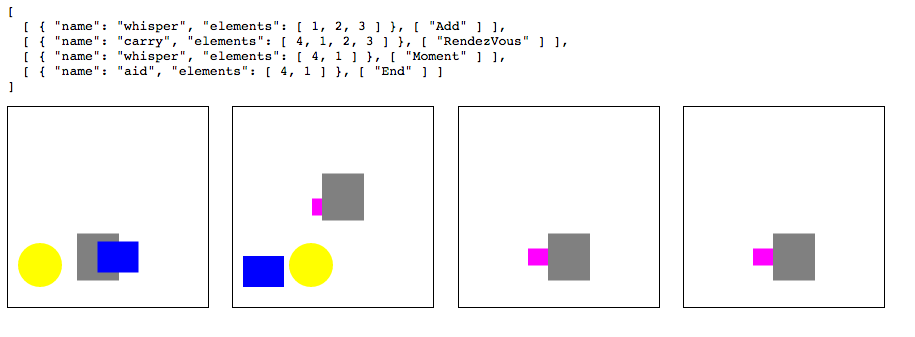
\includegraphics[width=0.5\textwidth]{comicgen-unconstrained-ok.png}
\label{fig:out1}
\end{figure}

\section{Constraining generation with Cohn grammars}

Generating random transition sequences may result in nonsensical output,
such as ending a comic with a ``meanwhile'' frame in which completely new
visual elements are introduced at the end of the comic, but not connected
back to previous elements; see Figure~\ref{fig:outbad} for an example. 

\begin{figure}
\caption{Example of underconstrained output.}
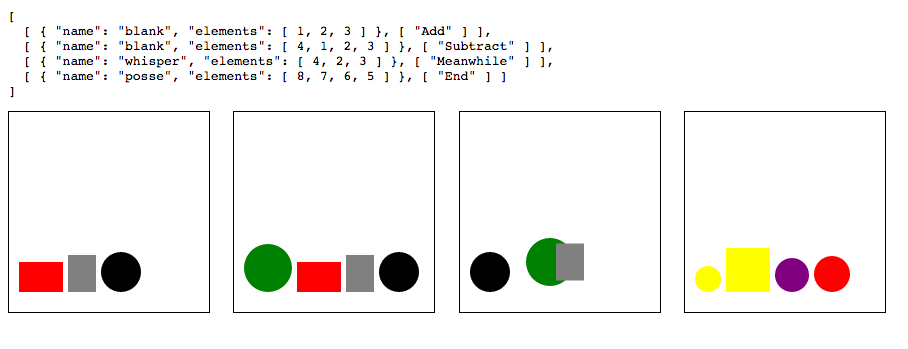
\includegraphics[width=0.5\textwidth]{comicgen-underconstrained-2.png}
\label{fig:outbad}
\end{figure}

In an attempt to understand the global structure of comic panel sequences,
Cohn et al. (XXX cite) investigate the {\em linguistic structure} of
visual narratives. They claim that understandable comics follow a grammar
that organizes its global structure. Instead of transition types, Cohn's
grammar of comics consists of {\em roles} that each panel plays in the
narrative. These roles are {\bf establisher}, {\bf initial}, {\bf
prolongation}, {\bf peak}, and {\bf release}, which allow the formation of
standard narrative patterns including the Western ``initial, peak,
release'' dramatic arc. Formally, Cohn gives the following grammar 
as a general template for sequences of panel roles:

{\it
(Establisher) -- (Initial (Prolongation)) -- Peak -- (Release)}

Symbols in parentheses are optional. In our expression of this grammar (and
in several of Cohn's examples), we also assume that prolongations may occur
arbitrarily many times in sequence.

Grossman built a generator based purely on Cohn's arc grammar,\footnote{
  \url{http://www.suzigrossman.com/fineart/conceptual/Sunday_Comics_Scrambler}
}
picking hand-annotated panels for each of an {\em initial},
{\em peak}, and {\em release} slot in the comic. However, this generation
scheme does not manipulate the internal structure of the comic panels,
allowing for less variability in the output than our scheme with visual
elements and frames. Additionally, codifying the syntactic structure of
individual panels allows us to characterize {\em relatedness} between
panels in the manner of Saraceni (XXX cite). In our second iteration of the
generator, we combine two approaches to discourse, using {\em global} Cohn
grammars to guide the {\em local} selection of syntactically-defined
transitions.

% What I want to say is: we don't just benefit from Cohn's work;
% he benefits from ours, because we're operationalizing semantic panel
% roles in terms of the panel's syntactic relationship to prior panels.
% I.e. in the linguistic metaphor, we're rejecting "panels as words" and
% instead treating "panels as utterances" and their constituent VEs as
% words.
% Maybe it's worth suggesting that panels themselves could obey a grammar,
% rather than haphazardly plugging VEs into different frame positions?

In particular, we enumerate every possible role bigram in Cohn's grammar,
such as {\em initial to prolongation}, {\em prolongation to peak}, and so
on, and describe sets of transition types that could plausibly model the
relationship. This mapping is determined by the code below:

\begin{Verbatim}[fontsize=\scriptsize]
let valid_transitions roles =
  match roles with
    (Establisher, Initial) -> 
      [Moment; Subtract; Add; RendezVous]
  | (Establisher, Prolongation) -> 
      [Moment; Subtract; Add]
  | (Establisher, Peak) -> [Add; Meanwhile]
  | (Initial, Prolongation) -> [Moment; Subtract; Add]
  | (Prolongation, Prolongation) -> 
      [Moment; Subtract; Add]
  | (Prolongation, Peak) -> [Subtract; Add; RendezVous]
  | (Initial, Peak) -> 
      [Subtract; Add; Meanwhile; RendezVous]
  | (Peak, Release) -> [Subtract; Add; RendezVous]
  | _ -> [End] (* error! *)
\end{Verbatim}

XXX describe randomly generating an instance of the grammar and feeding it
to the otherwise-same generator

Examples of the constrained generator's output can be found in
Figure~\ref{fig:outgood}.

\begin{figure}
\caption{Example of grammatically-constrained output.}

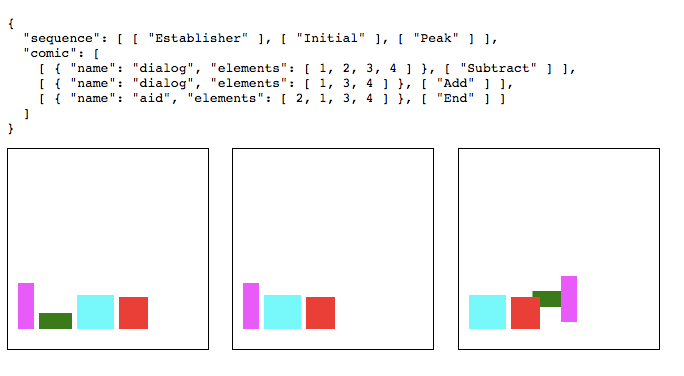
\includegraphics[width=0.5\textwidth]{comicgen-output-constrained-1.png}

Another example:

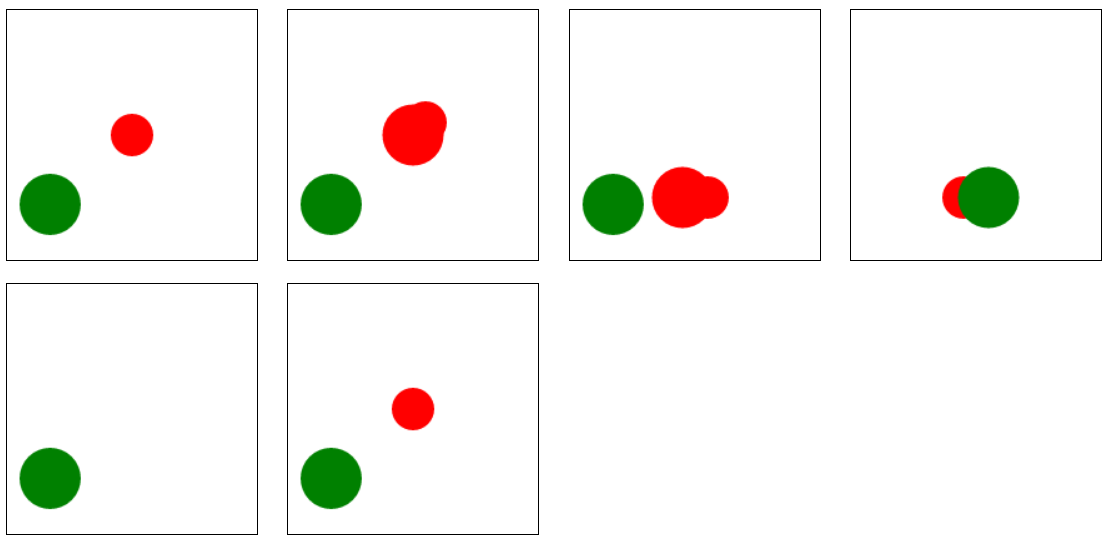
\includegraphics[width=0.5\textwidth]{comicgen-output-4.png}

\label{fig:outgood}
\end{figure}



